\section{Introduction}
A long-term goal of robotics research is the introduction of intelligent household robots.
To be effective, such a robot will need to perform complex tasks (e.g., setting a dinner table, doing laundry)
over long horizons. Planning for these long-horizon tasks is infeasible
for state-of-the-art motion planners, making apparent the need
for a hierarchical system of reasoning.

One way to approach hierarchical planning is through combined \emph{task and motion planning} (TAMP). In this
approach, an agent is given a symbolic, logical characterization of actions (e.g., move, grasp,
putdown), along with a geometric encoding of the environment. The hierarchical separation of high-level, symbolic task planning
from low-level, geometric motion planning enforces abstraction:
the task planner maintains no knowledge of the environment geometry, and the
motion planner has no understanding of the overall goal.
Efficient integration of these two types of reasoning is challenging, and recent research has
proposed several methods for it~\cite{srivastava2014combined, kaelbling2011hierarchical,
lagriffoul2014orientation, GarrettWAFR14, dornhege2012semantic}.

\begin{figure}[h]
  \centering
    \noindent
    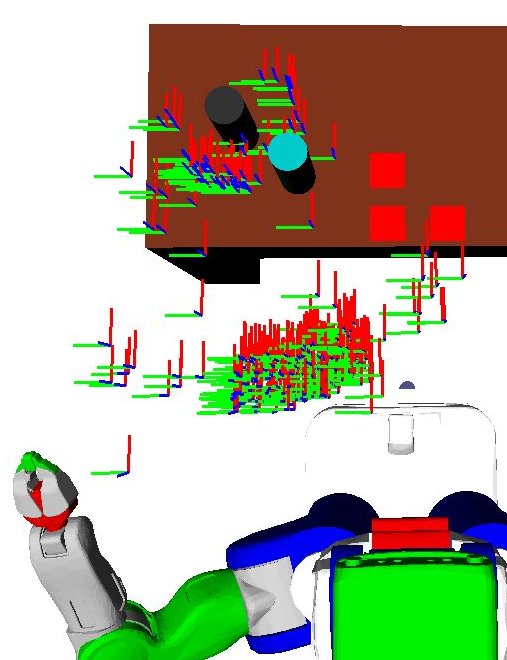
\includegraphics[scale=0.2]{images/move_grasp.png}\hspace{10 mm}
    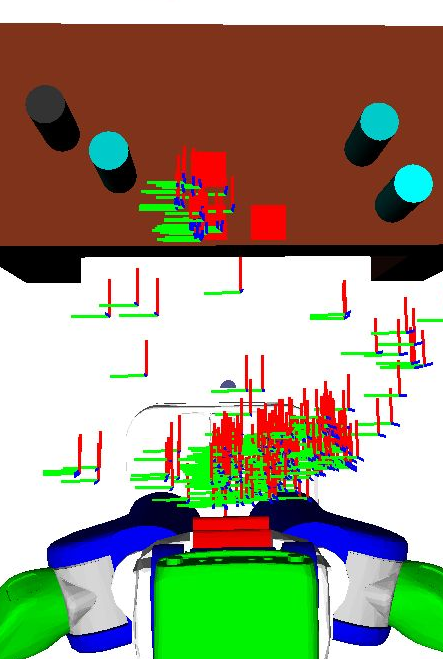
\includegraphics[scale=0.2]{images/move_putdown.png}
  \caption{Screenshots showing some distributions learned by our system in a simulated pick-place
    domain. We use reinforcement learning to train good distributions for sampling continuous parameters
    for motion planning. The robot is tasked with grasping the black cylinder and putting it down on the
    central red square. The left image shows learned base motion and grasping distributions,
    and the right shows learned base motion and putdown distributions. The grasp distribution
    properly learned to avoid the region close to the blue obstruction. These distributions are
    optimized to reduce the number of motion planning calls needed to produce a complete plan.}
  \label{fig:cover}
\end{figure}

A key limitation of TAMP systems is that they typically rely on hand-coded discretization to
sample continuous parameter values, such as target grasp poses, for motion planning.
These heuristic sampling distributions are tuned to the specific
geometric properties of the environment and its objects, and designing them well
requires substantial effort. This has several negative implications: the parameters of the
hand-coded distributions must be fine-tuned when running the system in a new setting, and the
resulting refinement distributions lack robustness. In this paper, we present a reinforcement
learning method to train good proposal distributions for sampling continuous parameter
values intelligently.

Our solution builds on the TAMP system
presented by Srivastava et al.~\cite{srivastava2014combined}.
A (classical) task planner produces a symbolic plan containing
a sequence of actions to reach a goal state. Then, in a process known as \emph{plan refinement},
candidate values are proposed for the continuous variables in this symbolic plan, thus grounding it.
These candidate values are then checked locally for feasibility by calling a motion planner.

The authors propose an \emph{interface layer} for refining the plan into a set
of collision-free trajectories; it performs an exhaustive
backtracking search over a hand-coded discrete set of candidate plan variable values. If a motion
planning feasible refinement is not found within the resource limit,
symbolic error information is propagated back to the task planner, and a new symbolic plan is produced.
The system uses an off-the-shelf classical task planner and motion planner, both as black boxes.
We build upon this framework because it is easy to separate the plan refinement module from the task planning module.
While our method is specific to this architecture, it can be adapted for other TAMP paradigms.

Reinforcement learning (RL) refers to the process of an agent learning a policy (a mapping from states to actions)
in its environment to maximize rewards. Zhang and Dietterich~\cite{JobShopSched} first applied the RL framework
to planning problems, using a job shop scheduling setting. In this work, we take inspiration from
their approach; we apply RL to plan refinement in a TAMP system. We implement our approach using methods adapted from
Zucker et al.~\cite{workspacebias}, who train a configuration space sampler for motion planning
using features of the discretized workspace. We train a policy that
determines how to sample values for symbolic plan parameters, using policy optimization with linear function
approximation. Our approach allows the learned distributions to be continuous, robust to changes in
the environment, and trainable for any experimental setting, eliminating the need for hand-tuned
distribution parameters.

The three contributions of our work are as follows:
\begin{tightlist}
\item[1)] We present randomized refinement,
a local search algorithm for plan refinement. Randomized refinement maintains at
all times a set of values for all symbolic plan variables, then at each iteration randomly
resamples one whose current instantiation is causing a failure. This naturally guides
plan variable resampling intelligently and easily lends itself to RL.
\item[2)] We describe how to formulate plan refinement (using randomized
refinement) in the RL framework, so that sampling
distributions for plan variables can be learned instead of hand-coded. Our formulation optimizes for
minimizing the number of calls to the motion planner.
\item[3)] We present experiments to evaluate our approach
in a variety of test environments involving complicated grasp and putdown
actions with obstructions and base motion.
\end{tightlist}
Our experimental results demonstrate that our approach is competitive with hand-coded discretization
of the plan refinement sample space, with respect to both motion planning time and number of calls
to the motion planner.